% Adapted from papers/zon/iclr2027_conference.tex.
\chapter[Adaptive Sparse Memory]{Adaptive Neural Activity Transformer}\label{ch:zon}

\definecolor{ratioMoE}{HTML}{7F5539}
\definecolor{ratioDenseA}{HTML}{9C6644}
\definecolor{ratioDenseB}{HTML}{B08968}
\definecolor{ratioDenseC}{HTML}{DDB892}
\definecolor{ratioDenseD}{HTML}{E6CCB2}

\section{Introduction}
Chapter~\ref{ch:mrl} showed that Matryoshka embeddings concentrate much of their
information in a low-dimensional subspace. This chapter extends the investigation to autoregressive
language models. We study redundancy in the intermediate activations of Transformer
MLPs and introduce \textbf{ZeroNeuron (ZoN)}, an input-dependent gate that selects
which intermediate coordinates to activate for each token. We then return to
embedding models to examine adaptive coordinate selection beyond vector slicing
as used in MRL.

As stated earlier, increasing LLM size improves performance but also raises training costs.
The question is how to train large models efficiently at a lower computational cost.
Sparsity, particularly MoEs, has emerged as an
effective solution for training large language models economically. In these models, the Transformer's
MLP is replaced by larger matrices, but only parts of them are activated for each input token.
MoEs can be viewed as activation sparsity applied to groups of channels: only a subset of
these groups is activated for each token. Keeping the total matrix size and sparsity fixed while reducing
the group size yields finer-grained sparsity, which has been shown to improve language
modeling \citep{krajewski2024scaling}. Taking this granularity to the extreme leads to an architecture similar to
a sparse memory layer \citep{he2024mixturemillionexperts, lample2019largememorylayersproduct}
roughly corresponding to one expert per channel.

A memory layer \citep{weston2015memorynetworks,lample2019largememorylayersproduct} 
stores trainable key-value pairs $(k_i,v_i)$, with $k_i\in\mathbb{R}^{d_q}$ and
$v_i\in\mathbb{R}^{n}$, but only a subset of pairs is used for computation for a given input token.
Given an input $x\in\mathbb{R}^{d}$, a query network
first produces $q(x)\in\mathbb{R}^{d_q}$. Each key receives a score
$s_i=q(x)^\top k_i$, measuring how well it matches the query.
The layer keeps only the $k$ keys with the largest scores.
We denote the indices of these selected keys by $\mathcal{I}$ and apply
$w=\mathrm{Softmax}((s_i)_{i\in\mathcal{I}})$ to obtain their weights.
Finally, the corresponding values are combined into the output
$m(x)=\sum_{i\in\mathcal{I}}w_i v_i$. Thus, the query determines which values
are retrieved and how much each contributes.

While appealing for achieving finer-grained sparsity, sparse memory layers
face several challenges. Selecting keys becomes expensive as the memory grows.
Approaches such as PKM \citep{lample2019largememorylayersproduct} 
and UltraSparse \citep{huang2025ultrasparsememorynetwork} reduce this cost through decomposition,
but TopK selection still adds computational cost as the candidate set grows.
When the memory is distributed across GPUs, tokens need to be sent to
the GPUs hosting their selected memory slots. 
TopK-based sparsity requires all-to-all communication, and these data transfers make sparse
memory layers communication-bound, especially when the memory spans many GPUs.
Moreover, the discrete selection made by TopK is not differentiable,
which can make routing harder to optimize at high levels of fine-grained sparsity.
Finally, TopK uses a fixed selection budget: every token activates the same number of
key-value pairs, regardless of the difficulty of the task.

We go beyond standard sparse memory designs and TopK with the following contributions:
\begin{enumerate}
    \item Leveraging the key-value memory interpretation of the MLP \citep{geva-etal-2021-transformer}, 
    we propose to make it sparse by learning to activate only the key-value pairs needed for each token.
    \item We motivate this approach by observing that MLP intermediate activations mostly lie
    in a subspace much smaller than the full available space.
    We show that granular MoE experts compress input representations into narrower
    spaces that their activations occupy more fully. These observations
    motivate learning to select which intermediate coordinates to activate.
    \item To select the needed key-value pairs for each token, we revisit stretching
    methods to learn activation sparsity in a way that is differentiable almost everywhere.
    The sparse gating is adaptive and applied pointwise, which is advantageous
    in distributed training as it allows each GPU to activate
    its local memory slots without needing to dispatch token representations as in TopK-based routing.
    This enables retaining the communication pattern of a dense tensor-parallel MLP in distributed training,
    which is simply an all-reduce and not the all-to-all in TopK-based activation sparsity.
\end{enumerate}
Section~\ref{sec:zon-memory} presents the key-value memory view and analyzes
intermediate activation rank in dense and sparse models.
Section~\ref{sec:zon-sparse_gating} introduces ZoN, and
Section~\ref{sec:zon-results} evaluates it in autoregressive language models.
Section~\ref{sec:zon-embedding_models} examines its extension to embedding models.

\section{Contemplating the MLP}\label{sec:zon-memory}
\subsection{Transformer MLPs as Key-Value Memories}
The MLP is defined by two linear
projections $\textbf{W}_{\text{k}} \in \mathbb{R}^{d_{\text{model}} \times d_{\text{inter}}}$, $\textbf{W}_{\text{v}} \in \mathbb{R}^{d_{\text{inter}} \times d_{\text{model}}}$:
\begin{align}
    \text{MLP}(\mathbf{x}) = \sigma(\mathbf{x} \textbf{W}_{\text{k}}) \textbf{W}_{\text{v}}.
\end{align}
where $\sigma$ is a non-linear activation function and $\mathbf{x} \in \mathbb{R}^{d_{\text{model}}}$ is the input token representation.
Modern architectures often use gated variants; we use this two-projection form to introduce the memory interpretation.
A possible interpretation of the MLP is to consider it as a key-value memory layer
\citep{geva-etal-2021-transformer,dai-etal-2022-knowledge,meng2023locatingeditingfactualassociations}.
$\mathbf{x}\textbf{W}_{\text{k}}$ scores how well the input matches each key.
The activation function \(\sigma\) transforms these scores into weights,
which are then used to aggregate the corresponding value entries in \(\mathbf{W}_{\mathrm{v}}\).
Usually, the dimension $d_{\text{inter}}$, called the \textit{intermediate dimension},
is much larger than $d_{\text{model}}$, often $4\times$, so it provides a large set of keys.
The kind of information stored in this memory remains an open research question.
Previous work found that these key-value pairs act as lexical dictionaries~\citep{geva-etal-2021-transformer},
where some keys are associated with specific lexical tokens.
Such associations can also reflect factual knowledge, as when a representation of ``The capital of France is'' retrieves information associated with ``Paris''.

If the MLP can be seen as a memory layer, it is arguable that this memory can be sparse,
since a given input may not need to activate all the key-value pairs.
It is conceivable that an input needs to retrieve only a subset of the key-value pairs.
If so, one could design a sparse activation gate that predicts ahead of time
which key-value memory pairs are needed for a given token representation.
But to motivate this approach, we first need to examine whether the intermediate activations contain redundancy
that a sparse gate could exploit. If so, we then need to design such a sparse gating function.

\subsection{The Effective Dimensionality of the MLP}
\label{sec:zon-rank_observations}
We analyze the eigenstructure of the MLP, both in dense and sparse models.

\begin{insightbox}{Observation 1: The MLP has low effective intermediate dimension}
Most activation energy is concentrated in a subspace with far fewer dimensions than the allocated intermediate space.
\end{insightbox}

\paragraph{Measuring the rank} We measure the effective dimensionality of the intermediate activations relative to their allocated width
$d_{\text{inter}}$ in dense and MoE Transformers.
We collect the key-projection activations before the nonlinearity using a calibration dataset $\mathcal{D}$.
For any input token $\mathbf{x} \in \mathcal{D}$, we define
$\mathcal{K} = \{ \mathbf{k} = \mathbf{x}\textbf{W}_{k} \}_{\mathbf{x} \in \mathcal{D}}$ with $\mathbf{k} \in \mathbb{R}^{d_{\text{inter}} }$.
We estimate the covariance matrix from these activations as
$\Sigma = \mathbb{E}[\mathbf{k}\mathbf{k}^\top] - \mathbb{E}[\mathbf{k}]\mathbb{E}[\mathbf{k}]^\top$.
We then compute the eigenvalues of this covariance matrix and sort
them in decreasing order, $\lambda_1 \geq \lambda_2 \geq \cdots \geq
\lambda_d$, where $d=d_{\text{inter}}$. We analyze the cumulative energy ratio $R(k)$, which is the
proportion of total activation variance explained by the top-$k$ eigenvalues:
\[
    R(k) = \frac{\sum_{i=1}^{k} \lambda_i}{\sum_{j=1}^{d} \lambda_j},
    \qquad k \in \{1,\ldots,d\}.
\]

    \begin{insightbox}{Observation 2: MoEs use smaller subspaces more fully}
    MoEs maintain a large total intermediate space, but each input
    token representation is projected into smaller subspaces.
    Activations occupy a larger fraction of the dimensions within these subspaces.
    \end{insightbox}

We report $R@p$, with $p \in [0,1]$, defined as the smallest fraction
$k/d$ such that $R(k) \geq p$. This ratio tells us how the activation energy is
spread. If the activations are low rank, $R(k)$ reaches $p$
more quickly, which means only a few dimensions are needed to represent most of
the activation energy. For example, if $R@1.0 = 0.4$, then about 40\% of the
dimensions are needed to represent all the activation energy. In practice,
because of numerical precision and small eigenvalue tails, reaching exactly
100\% can be unstable. We therefore use $p=0.99$ in our experiments.
Overall, the metric used is related to effective rank and stable rank, but
provides more flexibility by varying $p$.

\begin{table}[!htbp]
    \setlength{\abovecaptionskip}{3pt}
    \caption{We check possible sample size biases for Qwen3-30B-A3B, since
    MoE layers receive different numbers of tokens.
    We examine the correlation between the number of routed tokens
    per expert and the energy ratio $R@0.99$ and find none.}
    \label{tab:zon-moe_bias_checks}
    \centering
    \begin{tabularx}{\linewidth}{@{}Xr@{}}
    \toprule
    Metric & Value \\
    \midrule
    Mean $R@0.99$ across experts & 0.8318 \\
    Mean routed tokens per expert & 126{,}988 \\
    Median routed tokens per expert & 96{,}432 \\
    $\rho$ amount of routed tokens vs. ratio & 0.0799 \\
    \bottomrule
    \end{tabularx}
\end{table}

\paragraph{Results.} Figure~\ref{fig:zon-model_ratio99_activation} shows the percentage of dimensions needed to
represent 99\% of the activation energy. We can see that all dense models
have low effective dimension. This is also true for models with very low dimensions
such as Monad. The linear projection already limits the covariance rank to at most
$\min(d_{\text{model}},d_{\text{inter}})$, so expanding to $d_{\text{inter}}>d_{\text{model}}$
necessarily leaves linear dependencies among the intermediate coordinates.
Hence, the intermediate activations of dense models contain considerable redundancy.
As shown in Figure~\ref{fig:zon-model_ratio99_width}, fine-grained sparse MoEs reduce this redundancy
by projecting the input representation into different, smaller subspaces.
For example, Qwen3-30B-A3B has a total intermediate dimension of 98,304,
organized into 128 subspaces of 768 dimensions each.
Each token is projected into 8 of these subspaces.
Hence, the higher energy ratio of MoEs reflects fuller use of their smaller intermediate subspaces.
Since experts receive different numbers of tokens, we also check whether this affects
the measured ratio. For Qwen3-30B-A3B, Table~\ref{tab:zon-moe_bias_checks} shows negligible
linear correlation between the number of routed tokens and the ratio ($\rho=0.0799$).
These observations motivate an approach where the MLP intermediate dimension
is large but each token selects only the subspace it needs.

\begin{figure}[t]
\centering
\setlength{\abovecaptionskip}{2pt}
\pgfplotstableread[col sep=comma]{papers/zon/data/model_ratio99.csv}\ratiodata
% Keep the architecture table outside the plotting area.
\begin{minipage}[c]{0.54\linewidth}
\vspace{0pt}
\centering
\begin{tikzpicture}
\begin{axis}[
    width=\linewidth,height=5.5cm,font=\sffamily\scriptsize,
    ymin=0,ymax=1,xmin=-0.6,xmax=5.6,
    ylabel={Mean $R@0.99$},ytick={0,0.2,0.4,0.6,0.8,1},
    ymajorgrids,grid style={black!10},
    axis x line*=bottom,axis y line*=left,axis line style={black!60},
    xtick={0,1,2,3,4,5},
    xticklabels={{Qwen3\\30B\\A3B},{GPT\\OSS\\20B},{Monad\\57M},{Qwen3\\1.7B},{Qwen3\\4B},{Qwen3\\32B}},
    x tick label style={font=\sffamily\fontsize{6}{7}\selectfont,align=center,anchor=north},tick align=outside,
    ybar,bar width=15pt,nodes near coords,
    nodes near coords style={font=\sffamily\fontsize{6}{7}\selectfont,text=black},
    every node near coord/.append style={/pgf/number format/.cd,fixed,precision=2,fixed zerofill},
]
\newcommand{\rankbar}[3]{%
    \pgfplotstablegetelem{#1}{MeanRatio99}\of\ratiodata
    \edef\rankplot{\noexpand\addplot+[bar shift=0pt,fill=#3,draw=black!80]
        coordinates {(#2,\pgfplotsretval)};}%
    \rankplot
}
\rankbar{0}{0}{ratioMoE}
\rankbar{5}{1}{ratioDenseA}
\rankbar{1}{2}{ratioMoE!75!white}
\rankbar{2}{3}{ratioDenseB}
\rankbar{3}{4}{ratioDenseC}
\rankbar{4}{5}{ratioDenseD}

\end{axis}
\end{tikzpicture}
\end{minipage}\hfill
\begin{minipage}[c]{0.44\linewidth}
\centering
\scriptsize
\setlength{\tabcolsep}{2pt}
\renewcommand{\arraystretch}{1.2}
\resizebox{0.92\linewidth}{!}{%
\begin{tabular}{@{}lrrr@{}}
        \toprule
        Model & $d_{\text{model}}$ & $d_{\text{inter}}$ & $e_{\text{inter}}$ \\
        \midrule
        Qwen3-30B-A3B & 2048 & 98304 & 768 \\
        GPT-OSS-20B & 2880 & 92160 & 2880 \\
        Monad-57M & 256 & 768 & -- \\
        Qwen3-1.7B & 2048 & 6144 & -- \\
        Qwen3-4B & 2560 & 9728 & -- \\
        Qwen3-32B & 5120 & 25600 & -- \\
        \bottomrule
    \end{tabular}}
\end{minipage}
\caption[Effective intermediate dimension across models]{Mean $R@0.99$ across models, with model dimensions alongside.
Higher $R@0.99$ means that more activation components are needed to represent
99\% of the activation energy. For MoEs, $e_{\text{inter}}$ is the intermediate
dimension per expert and $d_{\text{inter}}$ is the total intermediate dimension
of the model.}
\label{fig:zon-model_ratio99_activation}
\label{fig:zon-model_ratio99}
\end{figure}

\begin{figure}[t]
\centering
\begin{minipage}{0.85\linewidth}
\vspace{0pt}
\centering
\begin{tikzpicture}
\begin{axis}[
    width=\linewidth,height=5.5cm,font=\sffamily\scriptsize,
    xlabel={$e_{\text{inter}}/d_{\text{model}}$},
    xmin=0.3,xmax=1.07,ymin=0,ymax=1,
    xtick={0.4,0.6,0.8,1},
    ytick={0,0.2,0.4,0.6,0.8,1},ymajorgrids,grid style={black!10},
    axis x line*=bottom,axis y line*=left,axis line style={black!60},
    tick align=outside,clip=false,
]
% Average the two Liquid models only for the connecting line.
\addplot[ratioMoE,line width=1.2pt] coordinates {
    (0.375,0.8317743937174479) (0.5,0.8135395050048828)
    (0.75,0.6788917054521276)
    (0.875,0.6796655658766693) (1,0.5262378833912037)
};
% All six measured values are retained as markers.
\addplot[only marks,mark=*,mark size=3.2pt,color=ratioMoE,
    mark options={fill=white,draw=ratioMoE,line width=0.8pt}]
    table[x=WidthRatio,y=MeanRatio99,col sep=comma]{papers/zon/data/moe_width_ratio99.csv};
% Dashed leaders link the labels to their hollow markers.
\node[anchor=south west,yshift=8pt,align=left,font=\sffamily\tiny,inner sep=1pt] (qwenlabel)
    at (axis cs:0.375,0.8317743937174479) {Qwen3\\30B-A3B};
\node[anchor=north east,yshift=-8pt,align=right,font=\sffamily\tiny,inner sep=1pt] (olmoelabel)
    at (axis cs:0.5,0.8135395050048828) {OLMoE\\1B-7B};
\node[anchor=north east,yshift=-8pt,align=right,font=\sffamily\tiny,inner sep=1pt] (glmlabel)
    at (axis cs:0.75,0.6788917054521276) {GLM-4.7\\Flash};
\node[anchor=south,yshift=8pt,align=center,font=\sffamily\tiny,inner sep=1pt] (lfmlabel)
    at (axis cs:0.875,0.6796655658766693) {LFM2/2.5\\8B-A1B};
\node[anchor=north east,yshift=-8pt,align=right,font=\sffamily\tiny,inner sep=1pt] (gptlabel)
    at (axis cs:1,0.5262378833912037) {GPT-OSS\\20B};
\begin{scope}[draw=ratioMoE,dash pattern=on 0.7pt off 0.9pt,line width=0.75pt,shorten >=0.5pt,shorten <=3.6pt]
\draw (axis cs:0.375,0.8317743937174479) -- (qwenlabel.south);
\draw (axis cs:0.5,0.8135395050048828) -- (olmoelabel.north);
\draw (axis cs:0.75,0.6788917054521276) -- (glmlabel.north);
\draw (axis cs:0.875,0.6796655658766693) -- (lfmlabel.south);
\draw (axis cs:1,0.5262378833912037) -- (gptlabel.north);
\end{scope}
\end{axis}
\end{tikzpicture}
\end{minipage}
\caption[Effective dimension and relative expert width]{Relationship between mean $R@0.99$ and relative expert width across six MoEs.
Ratios are measured within each expert, relative to $e_{\text{inter}}$.}
\label{fig:zon-model_ratio99_width}
\end{figure}

\section{Learning to Select Key-Value Pairs Adaptively}
\label{sec:zon-sparse_gating}
We showed that dense MLP activations occupy only part of the available intermediate space.
MoEs instead maintain a large total intermediate space, but each input token is projected
into smaller subspaces that are used more fully.
This motivates using a large intermediate dimension while selecting only the memory slots needed for each input token.
To avoid the fixed selection budget and token dispatch of TopK-based sparse memory layers,
we propose a new structured sparse gate that learns to zero out intermediate coordinates
for each input token.
\subsection{ZeroNeuron Sparse Activation Gating}
We revisit the hard-concrete distribution \citep{louizos2018learning}, originally
proposed to learn binary masks $\mathbf{z}$ for pruning. The core idea is to concentrate probability
mass at 0 and 1 through a ``stretching'' mechanism. It starts with a continuous relaxation
of Bernoulli sampling, producing values between 0 and 1, stretches them into the
interval $[l,r]$, where $l<0$ and $r>1$, and finally clips them back to $[0,1]$:
\begin{equation}
    \resizebox{\dimexpr\linewidth-3em\relax}{!}{$\displaystyle
    \begin{gathered}
    \mathbf{u}\sim\mathcal{U}(0,1),\quad
    \mathbf{s}=\operatorname{sigmoid}\big((\operatorname{logit}(\mathbf{u})+\log\boldsymbol{\alpha})/\beta\big),\quad
    \bar{\mathbf{s}}=\mathbf{s}(r-l)+l,\\[2pt]
    \mathbf{z}=\min(1,\max(0,\bar{\mathbf{s}})).
    \end{gathered}
    $}
\end{equation}
Here, $\boldsymbol{\alpha} \in \mathbb{R}_{>0}^{d_{\text{inter}}}$ are learnable parameters and $\beta>0$ is the temperature.
Clipping sets values below 0 to exactly 0 and values above 1 to exactly 1.
This makes the decision discrete by allowing some entries to be exactly switched on or off.
The reparameterized relaxation provides gradient estimates for learning the gates while allowing computation to be skipped where $\mathbf{z}_i = 0$. This approach has proven effective
for learning static pruning masks \citep{xia2024sheared, wang-etal-2020-structured}.

In order to learn predictive activation sparsity, we need to adapt this mechanism.
First, it was designed to learn a fixed pruning mask, while we want to predict which
coordinates to zero out based on the current input token.
Second, we want the active gates to remain continuous rather than being clipped to 1.
To address the first point, we predict $\log\boldsymbol{\alpha}$ with an input-dependent network.
To address the second, we apply stretching only on the left boundary ($0$).
Given an input $\textbf{x} \in \mathbb{R}^{d_{\text{model}}}$,
we define ZeroNeuron ${\mathrm{ZoN}}(\mathbf{x})$, a revised hard-concrete distribution, as:
\begin{equation}
    \resizebox{\dimexpr\linewidth-3em\relax}{!}{$\displaystyle
    \begin{gathered}
    \mathbf{u}\sim\mathcal{U}(0,1),\quad
    \mathbf{s}=\operatorname{sigmoid}\big((\operatorname{logit}(\mathbf{u})+\log\boldsymbol{\alpha}(\mathbf{x}))/\beta\big),\quad
    \bar{\mathbf{s}}=\mathbf{s}+l(1-\mathbf{s}),\\[2pt]
    \mathbf{z}=\max(0,\bar{\mathbf{s}}).
    \end{gathered}
    $}
\end{equation}
It is possible to encourage sparsity using $l_0$ regularization.
The expected number of active output coordinates has a differentiable closed form:
\begin{equation}
    \mathbb{E}\!\left[\|\mathbf{z}\|_0\right] = \sum_{i=1}^{d_{\text{inter}}}
    \operatorname{sigmoid}\!\left(\log\alpha_i(\mathbf{x})-\beta\log(-l)\right).
\end{equation}

Adding $\mathbb{E}[\|\mathbf{z}\|_0]$ to the training loss encourages fewer active coordinates.
Since $\mathbb{E}\!\left[\|\mathbf{z}\|_0\right]$ directly measures the expected number of active
coordinates, we can impose a target active intermediate dimension $h$ through a Lagrangian objective:
\begin{equation}
    \label{eq:zon-lg}
    \mathcal{L}_{\text{sparsity}} = \lambda_1 (\mathbb{E}\!\left[\|\mathbf{z}\|_0\right] - h) + \lambda_2 {(\mathbb{E}\!\left[\|\mathbf{z}\|_0\right] - h)}^2
\end{equation}
where $\lambda_1$ and $\lambda_2$ are the trainable Lagrangian scalar parameters.

The gate thus retains two useful properties of the hard-concrete distribution:
a differentiable objective for the expected number of active coordinates and a
pointwise sparsification process. The latter is beneficial for tensor parallelism,
as discussed below.

\subsection{Structured Activation Sparsity of the MLP}
\begin{lstlisting}[
  float=tb,
  language=Python,
  frame=tb,
  backgroundcolor=\color{black!3},
  rulecolor=\color{black!25},
  keywordstyle=\color{magenta!80!black}\bfseries,
  commentstyle=\color{green!55!black}\ttfamily,
  stringstyle=\color{violet!80!black},
  identifierstyle=\color{black},
  numbers=none,
  columns=fullflexible,
  keepspaces=true,
  showstringspaces=false,
  caption={Simplified implementation of the ZoN MLP training forward pass.},
  label={lst:zon-mlp}
]
import math
import torch

def mlp_zon(x, W_k, W_v, act_fn, a, beta=1.0, l=-0.01):
    """
    x: [batch * seq_len, d_model]
    W_k: [d_model, d_inter]
    W_v: [d_inter, d_model]
    a: gate network, d_model -> d_inter
    """
    log_alpha = a(x) # shape: [batch * seq_len, d_inter]

    # Sample gates
    u = torch.empty_like(log_alpha).uniform_(eps, 1 - eps)
    s = torch.sigmoid((torch.logit(u) + log_alpha) / beta)
    # stretch beyond zero and clamp to 0.0
    z = (s + l * (1 - s)).clamp(min=0.0)
    # Expected average of active gates per token
    avg_active = torch.sigmoid(
        log_alpha - beta * math.log(-l)
    ).mean()

    h = act_fn((x @ W_k) * z)
    o = h @ W_v

    return o, avg_active
\end{lstlisting}

Using the definition of the MLP as a key-value memory, we can write its sparsely activated version as:
\begin{align}
    \text{MLP}_{\text{ZoN}}(\mathbf{x}) = \sigma((\mathbf{x} \textbf{W}_{\text{k}}) \odot \mathbf{z}) \textbf{W}_{\text{v}}
\end{align}
where $\mathbf{z} \in \mathbb{R}^{d_{\text{inter}}}$ is the output of the sparse activation gate
$\mathbf{z} = {\mathrm{ZoN}}(\mathbf{x})$.
Since $\mathbf{z}$ predicts ahead of time which of the $d_{\text{inter}}$ coordinates to zero out
for this input token, it decides which key-value pairs to ignore. Hence,
the sparsity is structured and can be leveraged to accelerate training provided a GPU kernel can exploit this sparsity.
For the predicted sparsity to be used for sparse computation in both
$\textbf{W}_{\text{k}}$ and $\textbf{W}_{\text{v}}$, the non-linear activation
$\sigma$ must preserve zeros: $\sigma(0) = 0$. This ensures that coordinates
zeroed out by the gate remain zero after the activation. Fortunately, this holds
for common activations in modern Transformer MLPs, such as SiLU, ReLU, and
$\mathrm{ReLU}^{2}$.
Listing~\ref{lst:zon-mlp} provides a dense reference implementation of the gated MLP in PyTorch.
It computes both matrix multiplications densely; realizing computational savings
requires a kernel that skips the coordinates predicted to be inactive.

\subsubsection{Local and Global Sparsity Constraints}
While the provided implementation is illustrated on a single MLP layer, the Transformer
model has $L$ such MLP layers. Each has its own sparse gate.
The sparsity constraint can be applied either locally or globally. When applying
the sparsity constraint locally, each MLP layer converges to the specified
target sparsity.
In contrast, applying the constraint globally means that only the average
sparsity across layers is constrained. Individual layers can therefore use
different sparsity levels, allowing the model to allocate more active neurons to
layers that require greater capacity while inducing higher sparsity
in less demanding layers. This provides greater flexibility while maintaining
the desired overall compute budget. In our setting, we use a global sparsity
constraint for greater flexibility. Hence, we define
the average expected number of active gates across all $L$ MLP layers as
$\mathbb{E}_{\text{L}}\!\left[\|\mathbf{Z}\|_0\right] = \frac{1}{L} \sum_{l=1}^{L}\mathbb{E}_{l}\!\left[\|\mathbf{z}\|_0\right].$
Using $\mathbb{E}_{\text{L}}\!\left[\|\mathbf{Z}\|_0\right]$ as the expected sparsity in Equation~\ref{eq:zon-lg}
enforces the global sparsity constraint across all layers.

\subsubsection{Parameterizing the Gate Network}
The design of the gate network $\boldsymbol{\alpha}(\mathbf{x})$
is flexible: the network can be complex, non-linear, and deep. However,
its parameter count must remain manageable as the intermediate dimension grows.
We found that the gating network can be very small without hurting performance.
We parameterize the gate logits with a low-rank projection:
\begin{equation}
    \log\boldsymbol{\alpha}(\mathbf{x})
    = (\mathbf{x}\mathbf{A}_1)\mathbf{A}_2 + \mathbf{b}.
\end{equation}
Here, $\mathbf{A}_1\in\mathbb{R}^{d_{\text{model}}\times r}$ and
$\mathbf{A}_2\in\mathbb{R}^{r\times d_{\text{inter}}}$.
The bias $\mathbf{b}\in\mathbb{R}^{d_{\text{inter}}}$ controls the initial gate activity.
We found that a small rank is sufficient, so in our experiments we fix $r = d_{\text{model}} / 8$.
We do not yet understand why such small gating networks work well. One possible
explanation is that the sigmoid is applied independently to each coordinate, so
each gating decision can be made without modeling interactions among all
intermediate dimensions. In contrast, a softmax produces a probability
distribution jointly over the intermediate dimensions, which may require a
larger routing network to model these dependencies.

\subsubsection{On the efficiency of ZoN}
The proposed sparse activation gating offers several opportunities to reduce training and
inference costs relative to dense models and other TopK-based sparse models such
as MoEs and sparse memory layers.

First, the approach learns structured activation sparsity. The sparsity
emerges quickly during training and a sparse GPU kernel can exploit this to skip
computation of the zeroed-out coordinates to accelerate training and inference.
Given the predicted sparse gates $\mathbf{z} \in \mathbb{R}^{t \times d_{\text{inter}}}$ for $t$ tokens,
the corresponding predicted zero gates in $W_\text{k}$ and $W_\text{v}$ can be skipped
during the MLP forward and backward passes. There are many sparse GPU kernels in the literature
that can be adapted to accelerate training and inference, such as DejaVu
~\citep{liu2023dejavucontextualsparsity} or TEAL~\citep{TEAL}.

Second, the proposed sparsification approach is pointwise:
the sigmoid and stretching apply independently
to each coordinate. Compared to TopK-based activation sparsity,
this makes the approach less communication-bound in
distributed training, especially with tensor-parallel sharding.
Suppose the gates and the two MLP projections are sharded
along the intermediate dimension across $N$ GPUs.
Each GPU predicts its local gates from the same input $\mathbf{x}$ and applies
\texttt{zon\_mlp} using its local weights to compute its contribution
$\mathbf{y}_i$ to the output. An all-reduce then sums these contributions across
GPUs and gives each GPU the full output $\mathbf{y}=\sum_{i=1}^{N}\mathbf{y}_i$.
This is the same output communication used in a dense tensor-parallel MLP.
This approach therefore uses less communication than TopK-based
routing that needs to dispatch token representations to the
GPUs hosting their selected memory slots.

The main possible disadvantage of the proposed approach is
that different tokens can activate different MLP intermediate coordinates,
leading to scattered memory accesses for sparse computation.
This can make the computation memory-bandwidth-bound: reading the weights becomes
the bottleneck rather than performing the computation. One way to reduce this cost
is to group tokens that activate similar coordinates into buckets and process them
together. The benefit depends on how much their active coordinates overlap
and the cost of grouping the tokens.

\section{Experiments}
\label{sec:zon-results}

\subsection{Experimental Setup}
\paragraph{Implementation.}
Our experiments are based on nanochat, a minimalist GPT implementation optimized
for dense training. For fair comparisons, we keep the hyperparameter
settings unchanged, which have been optimized for dense models. Transformer matrices,
including the sparse gate network projections, are optimized with Muon.
The embeddings, the output head, biases, and scalar parameters use AdamW.
In each MLP, the gate network uses two linear projections with a bottleneck
of $d_{\text{model}}/8$ and a learned output bias. We set $\beta=1$ and $l=-0.01$.
The gates are initialized to keep almost all coordinates active at the beginning of training.
The gradient signal from the sparsity loss can be as strong as that from the language modeling
loss at the beginning of training.
We therefore introduce a sparsity ramp-up in which we leave sparsity unconstrained
for the first 1,000 steps, then linearly increase the target sparsity over 4,000 steps.
The constraint is applied to the average expected sparsity across layers,
with a Lagrange multiplier updated at each training step.
Gates are sampled during training and computed deterministically at evaluation.
\begin{table}[!htbp]
\caption{Model architecture and training budgets. Dense-600M uses a narrower MLP; the other architecture settings are shared.}
\label{tab:zon-architecture}
\begin{center}
\small
\setlength{\tabcolsep}{4pt}
\resizebox{\linewidth}{!}{%
\begin{tabular}{lccc}
\toprule
\textbf{Configuration} & \textbf{Dense-600M} & \textbf{Dense-1.2B} & \textbf{ZoN-1.2B-A600M} \\
\midrule
Total parameters & 600,834,122 & 1,233,125,450 & 1,233,125,450 \\
Transformer layers & \multicolumn{3}{c}{24} \\
Hidden dimension & \multicolumn{3}{c}{1,536} \\
Query heads & \multicolumn{3}{c}{12} \\
Key/value heads & \multicolumn{3}{c}{12} \\
MLP expansion multiplier & $2.417\times$ & \multicolumn{2}{c}{$8\times$} \\
MLP intermediate dimension & 3,712 & \multicolumn{2}{c}{12,288} \\
Vocabulary size & \multicolumn{3}{c}{32,768} \\
Context length & \multicolumn{3}{c}{2,048} \\
Sliding-window pattern & \multicolumn{3}{c}{\texttt{3:1}} \\
\midrule
Training tokens (approx.) & \multicolumn{3}{c}{13B} \\
\bottomrule
\end{tabular}}
\end{center}
\end{table}


\paragraph{Models.}
We train three models: Dense-600M, a 600M dense model, Dense-1.2B, a 1.2B dense model, and
ZoN-1.2B-A600M, a 1.2B model with 600M active parameters using our proposed approach.
All three models are trained on approximately 13B tokens, with their architecture
settings summarized in Table~\ref{tab:zon-architecture}. Dense-1.2B uses the same
MLP dimensions as ZoN-1.2B-A600M, while Dense-600M uses a narrower MLP to match its
approximate active parameter count. This setup helps us study whether, for the same number of
active parameters, increasing the total number of model parameters improves performance.

\paragraph{Evaluation.}
We use the DataComp-LM CORE evaluation setup
\citep{li2025datacomplmsearchgenerationtraining}, as implemented in nanochat.
The suite contains 22 tasks covering commonsense reasoning, reading comprehension,
language modeling, knowledge, and symbolic reasoning, with task-specific prompts
and few-shot settings. The evaluator scores multiple-choice and schema tasks by
selecting the answer with the highest average log-probability over the scored
continuation. For completion tasks, every target token must be the model's most
likely prediction given the preceding reference tokens. We report raw task accuracies
and the aggregate CORE score. To compute the aggregate CORE score, each
task accuracy $a$ is first centered as $(a-b)/(1-b)$, where $b$ is the task's random
baseline.

\subsection{Results}
\begin{table}[!htbp]
\caption{Benchmark accuracy (\%) for the dense and sparse models.
CORE reports the mean centered score (\%). BB denotes BIG-bench.}
\label{tab:zon-benchmarks}
\begin{center}
\small
\setlength{\tabcolsep}{2pt}
\resizebox{\linewidth}{!}{%
\begin{tabular}{@{}lccc@{}}
\toprule
\textbf{Benchmark (n-shot)} & \shortstack{\textbf{Dense}\\\textbf{600M}} & \shortstack{\textbf{Dense}\\\textbf{1.2B}} & \shortstack{\textbf{ZoN}\\\textbf{1.2B-A600M}} \\
\midrule
\multicolumn{4}{@{}l}{\textit{Commonsense reasoning}} \\
PIQA (10) & 74.37 & 76.93 & 75.35 \\
WinoGrande (0) & 56.91 & 60.30 & 60.77 \\
ARC-Easy (10) & 69.40 & 72.10 & 70.67 \\
ARC-Challenge (10) & 40.10 & 42.66 & 40.96 \\
HellaSwag (0) & 57.02 & 61.79 & 60.52 \\
HellaSwag (10) & 57.24 & 62.05 & 61.24 \\
\midrule
\multicolumn{4}{@{}l}{\textit{Commonsense reasoning and reading comprehension}} \\
COPA (0) & 66.00 & 64.00 & 68.00 \\
CommonsenseQA (10) & 21.38 & 32.02 & 28.67 \\
OpenBookQA (0) & 40.40 & 43.20 & 41.40 \\
Winograd (0) & 69.23 & 68.13 & 73.63 \\
BoolQ (10) & 61.62 & 63.79 & 61.31 \\
SQuAD (10) & 45.69 & 46.34 & 48.20 \\
\midrule
\multicolumn{4}{@{}l}{\textit{Reading comprehension, language modeling, and knowledge}} \\
CoQA (0) & 33.30 & 34.22 & 35.04 \\
LAMBADA (OpenAI) (0) & 43.22 & 46.81 & 46.96 \\
Jeopardy (10) & 9.40 & 15.21 & 15.07 \\
BB: QA Wikidata (10) & 46.44 & 51.30 & 50.51 \\
BB: Language identification (10) & 24.98 & 24.77 & 24.81 \\
AGI Eval: LSAT-AR (3) & 26.96 & 22.17 & 22.17 \\
\midrule
\multicolumn{4}{@{}l}{\textit{Symbolic reasoning}} \\
BB: Dyck languages (10) & 12.20 & 13.10 & 11.60 \\
BB: CS algorithms (10) & 44.32 & 39.39 & 44.32 \\
BB: Operators (10) & 18.57 & 17.62 & 19.05 \\
BB: Repeat copy logic (10) & 3.12 & 0.00 & 0.00 \\
\midrule
\rowcolor{ratioDenseD!40!white}
CORE & 27.3510 & 29.6130 & 29.7722 \\
\bottomrule
\end{tabular}}
\end{center}
\end{table}



\begin{figure}[t]
    \centering
    \subfloat[Target sparsity schedule with the delay and linear ramp phases.\label{fig:zon-rampup}]{\begin{minipage}{0.48\linewidth}
\centering
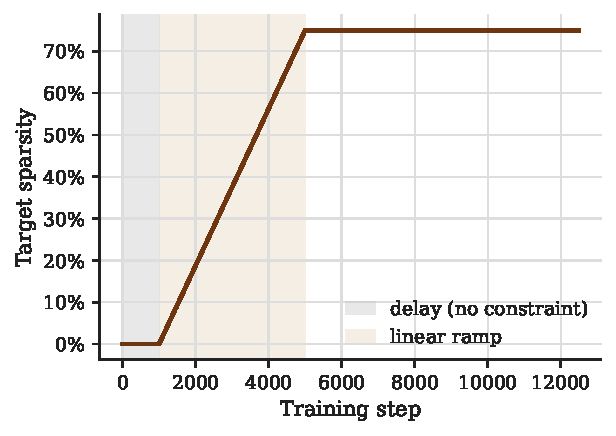
\includegraphics[width=\linewidth]{papers/zon/figures/figs/sparsity_rampup.pdf}
\end{minipage}}
    \hfill
    \subfloat[The convergence of the expected sparsity.\label{fig:zon-expected_sparsity}]{\begin{minipage}{0.48\linewidth}
\centering
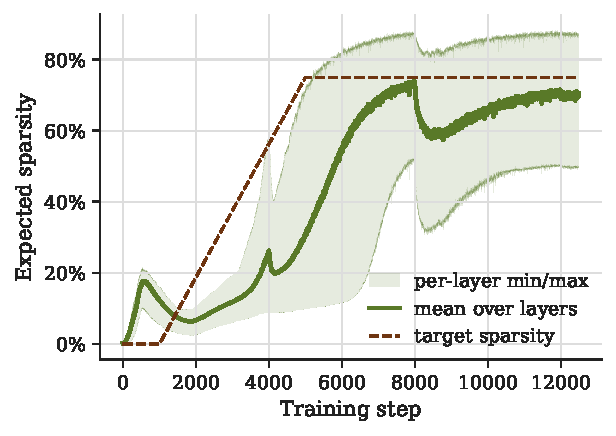
\includegraphics[width=\linewidth]{papers/zon/figures/figs/expected_sparsity.pdf}
\end{minipage}}
    \caption{Training dynamics of the adaptive ZoN gate.}
    \label{fig:zon-training_dynamics}
\end{figure}

Table~\ref{tab:zon-benchmarks} shows that ZoN-1.2B-A600M reaches a CORE score of
29.77, compared with 29.61 for Dense-1.2B and 27.35 for Dense-600M.
ZoN therefore achieves similar aggregate performance to the larger dense model
while using roughly 600M active parameters per token. Compared with the dense
model of similar active size, it improves CORE by 2.42 percentage points.
This supports the idea that keeping a larger memory and selecting which parts
to activate in the intermediate dimension can be more effective than using a smaller dense memory.

The comparison with Dense-600M is consistent across many tasks. For example,
ZoN improves HellaSwag accuracy from 57.24\% to 61.24\%, CommonsenseQA from
21.38\% to 28.67\%, and QA Wikidata from 46.44\% to 50.51\%.
Compared with Dense-1.2B, ZoN performs better on
Winograd and SQuAD, but worse on PIQA, ARC-Challenge, and CommonsenseQA.
Hence, the small CORE difference of 0.16 percentage points between the dense and sparse
1.2B models reflects comparable overall performance rather than a
consistent advantage over the larger dense model.

As described above, we gradually increase the target sparsity during training
to let the model focus on language modeling at the beginning.
Figure~\ref{fig:zon-rampup} shows this schedule, while
Figure~\ref{fig:zon-expected_sparsity} shows that the expected sparsity closely
follows it. This suggests that suitable sparse kernels could accelerate
training once sparsity emerges. For longer training runs, the same delay and
ramp would account for a smaller fraction of the total training steps.
The sparsity constraint applies to an average over input tokens, so individual
tokens and tasks can have different sparsity levels.
The reported sparsity of approximately 70\% is an average across evaluation tasks.
Table~\ref{tab:zon-tasks} reports the predicted sparsity (Zero frac.) for each
task, along with the centered accuracies used to compute the CORE metric.
\begin{table}[!htbp]
\caption{Evaluation of Dense-1.2B (Dense) and ZoN-1.2B-A600M (Sparse). All entries are percentages;
CORE is the mean centered score. $\%0$ measures the fraction of zeros predicted by ZoN
MLP gates during inference. BB denotes BIG-bench.}
\label{tab:zon-tasks}
\begin{center}
\small
\setlength{\tabcolsep}{4pt}
\resizebox{\linewidth}{!}{%
\begin{tabular}{lrrrrr}
\toprule
& \multicolumn{2}{c}{Accuracy} & \multicolumn{2}{c}{Centered} & Predicted $\%0$. \\
\cmidrule(lr){2-3}\cmidrule(lr){4-5}
Task & Dense & Sparse & Dense & Sparse & Sparse \\
\midrule
HellaSwag (zero-shot) & 61.79 & 60.52 & 49.05 & 47.35 & 69.19 \\
Jeopardy & 15.21 & 15.07 & 15.21 & 15.07 & 65.20 \\
BB: QA Wikidata & 51.30 & 50.51 & 51.30 & 50.51 & 65.30 \\
ARC-Easy & 72.10 & 70.67 & 62.79 & 60.89 & 69.56 \\
ARC-Challenge & 42.66 & 40.96 & 23.55 & 21.27 & 69.40 \\
COPA & 64.00 & 68.00 & 28.00 & 36.00 & 67.41 \\
CommonsenseQA & 32.02 & 28.67 & 15.03 & 10.83 & 71.84 \\
PIQA & 76.93 & 75.35 & 53.86 & 50.71 & 69.14 \\
OpenBookQA & 43.20 & 41.40 & 24.27 & 21.87 & 68.05 \\
LAMBADA (OpenAI) & 46.81 & 46.96 & 46.81 & 46.96 & 66.17 \\
HellaSwag & 62.05 & 61.24 & 49.40 & 48.32 & 68.29 \\
Winograd & 68.13 & 73.63 & 36.26 & 47.25 & 67.09 \\
WinoGrande & 60.30 & 60.77 & 20.60 & 21.55 & 66.98 \\
BB: Dyck languages & 13.10 & 11.60 & 13.10 & 11.60 & 75.95 \\
AGI Eval: LSAT-AR & 22.17 & 22.17 & 2.72 & 2.72 & 72.12 \\
BB: CS algorithms & 39.39 & 44.32 & 39.39 & 44.32 & 73.14 \\
BB: Operators & 17.62 & 19.05 & 17.62 & 19.05 & 73.53 \\
BB: Repeat copy logic & 0.00 & 0.00 & 0.00 & 0.00 & 70.89 \\
SQuAD & 46.34 & 48.20 & 46.34 & 48.20 & 67.87 \\
CoQA & 34.22 & 35.04 & 34.22 & 35.04 & 68.45 \\
BoolQ & 63.79 & 61.31 & 4.72 & -1.80 & 67.76 \\
BB: Language identification & 24.77 & 24.81 & 17.24 & 17.28 & 67.62 \\
\midrule
CORE & --- & --- & 29.6130 & 29.7722 & --- \\
\bottomrule
\end{tabular}}
\end{center}
\end{table}


\section{Generalization to Embedding Language Models}
\label{sec:zon-embedding_models}

We apply the same principle to embedding language models, using ZoN to predict
which coordinates of an embedding to keep. Here, we use NV-Embed representations
and train the gates without a specific target sparsity constraint. Unlike the MLP setting, we
stretch on both the left and right sides and clip the gates to $[0,1]$, encouraging
gates to be either zero or one. Binary masks can reduce the storage cost of the gates in a vector store; storing sparse embeddings also requires identifying their active coordinates. At inference, we keep the $k$ coordinates with
the highest sigmoid gate scores, with $k\in\{128,256\}$ for evaluation,
but $k$ can be chosen freely during inference, depending on the budget.

\paragraph{Experimental setup.}
For retrieval, we train a linear projector of shape
$d_{\text{model}}\times d_{\text{model}}$ on top of the embeddings, alongside
the gate projector. For classification, we instead use a two-layer perceptron,
with linear projections from $d_{\text{model}}$ to $4d_{\text{model}}$ and back to $d_{\text{model}}$,
with a ReLU activation between them. In both settings, the gate network uses
a hidden dimension of $r=d_{\text{model}} / 4$, with $d_{\text{model}}$ being
4096 for NV-Embed.
We evaluate retrieval on NFCorpus and SciFact using NDCG@10, and classification
on MTOPIntent and Banking77 using top-1 accuracy. We train for 10 epochs on
each dataset, except NFCorpus, where we use 2 epochs due to the training budget.

\begin{table}[!htbp]
\centering
\caption{Performance of NV-Embed representations on classification and retrieval
tasks. Scores are percentages. $k$ is the number of coordinates retained at
inference; dense representations use all $d_{\text{model}}$ coordinates.
The dense baseline uses NV-Embed with a projector fine-tuned on each task
and retains all coordinates. The best score in each column is bold and the second-highest
distinct score is underlined.}
\label{tab:zon-embedding_results}
\small
\setlength{\tabcolsep}{3pt}
\resizebox{\linewidth}{!}{%
\begin{tabular}{llc|cc|cc}
\toprule
& & & \multicolumn{2}{c|}{\textbf{Classification}} & \multicolumn{2}{c}{\textbf{Retrieval}} \\
& & & \multicolumn{2}{c|}{Top-1 Acc. (\%) $\uparrow$} & \multicolumn{2}{c}{NDCG@10 (\%) $\uparrow$} \\
\cmidrule{4-5}\cmidrule{6-7}
Category & Method & Dim. & MTOPIntent & Banking77 & NFCorpus & SciFact \\
\midrule
Dense & Fine-tuned & $4096$ & \underline{93.96} & \underline{93.73} & 55.01 & \textbf{84.87} \\
\midrule
& CSR & 256 & \textbf{96.85} & \textbf{94.38} & \textbf{56.12} & 73.20 \\
& CSR & 128 & \textbf{96.85} & \textbf{94.38} & 54.64 & 73.20 \\
\cmidrule{2-7}
\rowcolor{ratioDenseD!40!white}
\cellcolor{white} & ZoN (ours) & 256 & 91.68 & 92.93 & \underline{55.46} & \underline{82.06} \\
\rowcolor{ratioDenseD!40!white}
\cellcolor{white}\multirow{-4}{*}{Sparse} & ZoN (ours) & 128 & 90.04 & 91.02 & 52.14 & 81.23 \\
\bottomrule
\end{tabular}}
\end{table}


\paragraph{Results.}
We compare with CSR, a sparse-coding approach~\citep{wen2025matryoshkarevisitingsparsecoding}, discussed in Chapter~\ref{ch:mrl}.
Table~\ref{tab:zon-embedding_results} shows that the benefit depends on the task.
On SciFact, ZoN outperforms CSR, but remains below the full
fine-tuned representation. On NFCorpus, ZoN with $k=256$ slightly exceeds
the full fine-tuned representation, while CSR is better overall.
For classification, ZoN remains below both CSR and the baseline using NV-Embed
with a projector fine-tuned on the task and all embedding coordinates retained.
Increasing $k$ from 128 to 256 improves ZoN on all four tasks.
These results suggest that adaptive coordinate selection can preserve much
of the retrieval performance.

\section{Conclusion}
This chapter introduced ZeroNeuron, an input-dependent sparse gate motivated by the
key-value memory interpretation of Transformer MLPs. The rank analysis showed that
dense intermediate activations occupy only a fraction of their available space,
whereas fine-grained MoE experts use their smaller subspaces more fully. ZoN learns
to select individual intermediate coordinates while constraining the average number
of active gates across layers and tokens. At approximately 600M active parameters per token, ZoN-1.2B-A600M achieves a CORE
score of 29.77, comparable to 29.61 for Dense-1.2B and above 27.35 for Dense-600M.
The embedding experiments further show that adaptive coordinate selection can
preserve much of the retrieval performance.

Together with Chapter~\ref{ch:mrl}, these results conclude the activation-sparsity
part of the thesis: representational capacity need not be used uniformly for every
input. Learned adaptive activation sparsity allows the amount of sparsity to depend on the input.
Turning this flexibility into reliable runtime gains requires sparse implementations that exploit the learned
activation patterns efficiently.
